\chapter{Аналитическая часть}

\section{Введение в большие языковые модели}

Большие языковые модели (Large Language Models, LLM) представляют собой один из наиболее значимых прорывов в области обработки естественного языка (Natural Language Processing, NLP) за последние годы. 
Они используются для решения широкого спектра задач: от генерации текстов и перевода до извлечения информации и анализа тональности. 
В этой части мы подробно рассмотрим, что такое LLM, как они работают и какие модели получили наибольшее признание в научном и практическом сообществе.

\subsection{Определение LLM}

Большие языковые модели — это нейронные сети, обученные на огромных объёмах текстовой информации, способные понимать, генерировать и обрабатывать естественный язык. 
Ключевой особенностью этих моделей является их масштаб: количество параметров (веса, которые настраиваются во время обучения) может достигать сотен миллиардов, 
что позволяет моделям захватывать сложные языковые закономерности.

Формально, можно представить LLM как функцию:
\[
f_\theta: X \rightarrow Y, 
\]
где
\(X\) -- входная последовательность текста (например, набор слов или токенов),
\(Y\) -- выход модели, который может представлять собой продолжение текста, предсказание следующего слова или метки для классификации,
\(\theta\) -- вектор параметров модели, оптимизируемый в процессе обучения.

Одной из самых популярных архитектур, лежащих в основе современных LLM, является трансформер. 
Архитектура трансформера позволяет моделям обрабатывать все входные данные параллельно, 
что существенно ускоряет обучение и повышает качество обработки длинных последовательностей. 

Ключевые компоненты архитектуры трансформера включают:
\begin{itemize}
    \item 
    механизм внимания (attention): 
    позволяет модели взвешивать вклад каждого элемента входной последовательности при формировании выходного представления. 
    Простейший вариант -- механизм самовнимания (self-attention), где каждый токен оценивается относительно всех остальных токенов;
    \item
    многоголовочное внимание (Multi-head Attention): 
    позволяет модели одновременно фокусироваться на различных аспектах информации, что улучшает её способность учитывать сложные зависимости между токенами;
    \item
    нормализация и позиционные кодировки: 
    поскольку трансформеры не обладают врождённой способностью учитывать порядок слов, вводятся специальные позиционные кодировки, 
    которые позволяют модели учитывать последовательность входных данных.

\end{itemize}
    
\section{Принципы работы LLM}

Чтобы понять, как работают большие языковые модели, важно ознакомиться с несколькими базовыми понятиями.

\subsection{Токенизация} 

Токенизация – это процесс разбиения входного текста на более мелкие единицы, называемые токенами. 
Токен может быть словом, частью слова или даже символом. 
Например, фраза «Программное обеспечение» может быть разбита на два токена «Программное» и «обеспечение», 
либо на более мелкие единицы (например, корни, приставки, суффиксы) в зависимости от выбранного метода токенизации.

\subsection{Эмбеддинги}

После токенизации каждому токену присваивается эмбеддинг — вектор фиксированной размерности, который численно представляет смысл и контекст токена. 
Эмбеддинги позволяют модели работать с текстовыми данными, преобразовывая их в числовую форму, пригодную для дальнейшей обработки нейронной сетью. 
Обычно эмбеддинги обучаются одновременно с остальными параметрами модели или инициализируются с помощью предварительно обученных векторных представлений (например, Word2Vec \cite{lib:word2vec}).

\subsection{Механизм внимания и векторы контекста}

Основой работы трансформеров является механизм внимания. 
Его суть заключается в том, что при обработке каждого токена модель оценивает, насколько важен каждый другой токен в последовательности для определения его значения. 
Это позволяет учитывать долгосрочные зависимости, что особенно важно для понимания сложных синтаксических конструкций и контекстуальных взаимосвязей.

Процесс самовнимания можно формализовать следующим образом. 
Пусть \(Q\) (query), \(K\) (key) и \(V\) (value) – это матрицы, полученные из эмбеддингов токенов посредством линейных преобразований. 
Тогда механизм внимания рассчитывается по формуле:
\[
\text{Attention}(Q, K, V) = \text{softmax}\left(\frac{QK^T}{\sqrt{d_k}}\right)V,
\] 
где
T - операция транспонирования,
\(d_k\) – размерность векторов ключей,
\(\text{softmax}\) обеспечивает нормировку весов внимания, так что сумма их значений равна 1 \cite{lib:attention_is_all_you_need}.

Таким образом, каждая позиция в последовательности получает взвешенное представление, учитывающее информацию со всех остальных позиций, что и формирует вектор контекста.

\subsection{Генерация текста и предсказание следующего слова}

Одна из основных задач больших языковых моделей (LLM) – предсказание следующего слова в последовательности. Для этого модель сначала вычисляет логиты — необработанные оценки для каждого слова из словаря, а затем преобразует их в вероятностное распределение, используя функцию softmax. Это позволяет определить вероятность появления каждого слова в качестве следующего.
Функция softmax записывается следующим образом:
\[
softmax(z)_{i} = \frac{\exp\left(\mathbf{z}_{i}\right)}{\sum_{j} \exp\left(\mathbf{z}_i\right)},
\]
где
$z_{i}$ -- логит (необработанная оценка) для $i$-го слова в словаре,
$\exp({z}_{i})$ -- экспоненциальное преобразование логита, которое гарантирует положительные значения,
$\sum_{j} \exp(\mathbf{z}_i)$ -- сумма экспоненциальных значений всех логитов, служащая для нормализации, так что сумма вероятностей по всем словам равна 1 \cite{anal:softmax}.

\subsection{Prompt Engineering}

Prompt engineering — это искусство создания эффективных входных запросов (промтов) для LLM, чтобы направить их на выполнение конкретных задач. 
Промты могут включать инструкции, примеры, а также специфическую терминологию, которая помогает модели сконцентрироваться на нужном аспекте задачи. 

\section{Методы и алгоритмы извлечения информации}

Извлечение информации (Information Extraction, IE) из текстовых данных представляет собой процесс автоматизированного структурирования 
неформатированного текста путём выделения значимых элементов. 
К таким элементам относятся именованные сущности (например, персоналии, организации, локации), связи между ними, события и временные характеристики. 

\subsection{Обзор задач извлечения информации}

Ключевые задачи IE ориентированы на преобразование текста в структурированные форматы, что критически важно для последующего анализа. Основные направления включают:

\begin{itemize}
    \item распознавание именованных сущностей (Named Entity Recognition, NER): идентификация и классификация объектов текста по предопределённым категориям. Например, в предложении «Компания Tesla начала поставки электромобилей в Европу в марте 2023 года» система NER выделит «Tesla» (организация) и «Европу» (географический объект). Точность NER влияет на качество последующих этапов;

    \item извлечение отношений (Relation Extraction, RE): определяется семантическая связь между сущностями. Например, между «Tesla» и «Европой» устанавливается отношение, указывающее на направление поставок;

    \item извлечение временной информации (Temporal Information Extraction, TIE): распознаются временные выражения и приводятся к конкретному формату. Здесь временной указатель «в марте 2023 года» позволяет определить дату события.

    \item извлечение событий (Event Extraction, EE): выявляется событие и его компоненты. Из этого предложения можно извлечь событие начала поставок, где субъектом выступает «Компания Tesla», действием — «начала поставки», а объектом — «электромобили», с указанием времени «в марте 2023 года»;
\end{itemize}

\subsection{NER модели}

Модели распознавания именованных сущностей (NER) являются одним из центральных компонентов систем извлечения информации. 
Их основная задача — автоматическая идентификация и классификация объектов текста (персоны, организации, локации и т.д.) по заранее определённым категориям.
Существуют различные подходы к построению NER-моделей: основанные на правилах, использующие лингвистические правила и словари; основанные на машинном обучении (включая классические методы, такие как скрытые марковские модели и условные случайные поля, а также нейросетевые модели); и гибридные, комбинирующие оба подхода.

Среди нейросетевых моделей, демонстрирующих наиболее высокие результаты, выделяют рекуррентные нейронные сети (RNN, в частности, LSTM и GRU), 
сверточные нейронные сети (CNN) и трансформеры (BERT, RoBERTa, XLNet, ELECTRA и др.). 
Модели на основе правил отличаются высокой точностью при условии качественной проработки правил, но ограничены в обработке неоднозначности и новых слов. 
Модели машинного обучения, особенно нейросетевые, лучше справляются с неоднозначностью, способны к автоматическому извлечению признаков и обучению на больших объемах данных, однако требуют значительных вычислительных ресурсов и, как правило, менее интерпретируемы. 
Гибридные модели позволяют использовать преимущества обоих подходов.

\subsection{Современные подходы на основе LLM}

Большие языковые модели, предобученные на корпусах в масштабе терабайтов, кардинально изменили подходы к IE. Их ключевое преимущество — способность к контекстуальному пониманию, что критично для многозначных слов и имплицитных связей.

\subsubsection{Стратегии применения LLM}

\begin{itemize}
    \item Zero-shot вывод: модель выполняет задачу, используя только текстовое описание в промпте (например, «Извлеки все организации из текста»). Это удобно для быстрого прототипирования, но точность зависит от способности модели декодировать неявные инструкции. Например, LLM может спутать формат даты «05/06/2023» (5 июня на 6 мая) без явных указаний.

    \item Few-shot вывод: модель получает несколько примеров ввода-вывода, что особенно полезно для задач с нестандартными форматами.
    
    \item Дообучение (Fine-tuning): предобученная модель (например, BERT) адаптируется к конкретной задаче на размеченных данных. Для NER последний слой BERT заменяется на классификатор меток токенов.

    \item Специализированные LLM: модели вроде LUKE (обучена на связях между сущностями) или SPECTER (для научных текстов) используют доменно-специфичное предобучение.
\end{itemize}

\section{Существующие продукты на основе ИИ для анализа акторов, действий и временных характеристик}

Современные решения для извлечения акторов, действий и временных параметров из текста охватывают широкий спектр технологий. Ниже представлен анализ 30 ключевых продуктов, демонстрирующих разнообразие подходов в этой области.

\subsection{Популярные LLM}

\subsubsection{GPT-4 (OpenAI)}

GPT-4 (Generative Pre-trained Transformer 4) \cite{lib:chatgpt} представляет собой дальнейшее развитие авторегрессионной архитектуры OpenAI. 
Модель отличается улучшенной способностью к пониманию контекста, более глубоким семантическим анализом и генерацией текста повышенного качества. 
GPT-4 распространяется по закрытой коммерческой лицензии и доступна через API OpenAI, что требует оплаты и соблюдения установленных правил использования.

\subsubsection{BERT (Google)}

BERT (Bidirectional Encoder Representations from Transformers) \cite{lib:bert}  — модель, разработанная компанией Google, которая базируется на двунаправленной архитектуре трансформера. В отличие от авторегрессионных моделей, BERT обучается предсказывать маскированные слова в предложении с учетом контекста с обеих сторон, что делает её эффективной для задач, требующих глубокого понимания семантики текста. Модель является открытой и доступна для свободного использования и модификации, что способствует её широкому применению в академических и практических проектах. Благодаря двунаправленному обучению, BERT достигает высокой точности в таких задачах, как распознавание именованных сущностей (NER), извлечение отношений (RE), построение вопросно-ответных систем и классификация текста.

\subsubsection{LaMDA (Google)}

LaMDA (Language Model for Dialogue Applications) \cite{lib:lambda} — специализированная языковая модель, разработанная Google для создания диалоговых систем. Модель оптимизирована для ведения естественных и осмысленных бесед, поддержания контекста диалога и генерации релевантных ответов. Доступ к LaMDA ограничен и предоставляется преимущественно в рамках внутренних проектов Google или через партнёрские программы, что обусловлено стратегическими соображениями и необходимостью контроля за использованием модели. LaMDA обладает способностью поддерживать продолжительные и связные диалоги, адаптироваться к стилю общения собеседника и генерировать ответы с учётом предыдущих реплик, демонстрируя высокий уровень эмпатии.

\subsubsection{Gemini (Google)}

Gemini \cite{lib:gemini} — это семейство мультимодальных больших языковых моделей (LLM), разработанных Google. Способны обрабатывать и генерировать не только текст, но и изображения, аудио и видео. Gemini представлен в нескольких версиях (Ultra, Pro, Nano), оптимизированных для разных задач и устройств, от мощных серверов до мобильных телефонов. Gemini интегрирован в различные продукты Google, такие как поисковая система, рекламные сервисы и инструменты для разработчиков. Доступ к Gemini осуществляется через API и платформу Google AI Studio.

\subsubsection{Claude 2 (Anthropic)}
Claude 2 \cite{lib:Claude} — это модель, разработанная с использованием подхода «конституционального ИИ», направленного на обеспечение безопасного, полезного и этически корректного взаимодействия с пользователями. Модель доступна через API и оснащена механизмами фильтрации контента, предотвращающими генерацию нежелательных или опасных ответов.

\subsubsection{PaLM (Google)}

PaLM (Pathways Language Model) \cite{lib:palm} — масштабируемая языковая модель от Google, отличающаяся высокой производительностью и способностью обрабатывать огромные объёмы текстовых данных с высокой точностью. Модель использует архитектуру Pathways, которая эффективно распределяет вычислительную нагрузку между различными компонентами системы. PaLM распространяется по закрытой коммерческой лицензии и используется преимущественно в рамках внутренних проектов Google или через платные сервисы. Благодаря своей универсальности, PaLM успешно решает широкий спектр задач, включая обработку естественного языка, машинное обучение и анализ данных, демонстрируя выдающиеся результаты в задачах, требующих глубокого понимания контекста.

\subsubsection{DeepSeek}

DeepSeek \cite{lib:DeepSeek} представляет собой семейство языковых моделей, специализированных на задачах семантического поиска и извлечения информации. Модели DeepSeek способны обрабатывать запросы с учётом глубокого контекстного анализа, что делает их эффективными для построения поисковых систем и систем рекомендаций. DeepSeek распространяется с открытым исходным кодом, что позволяет свободно интегрировать её в исследовательские и коммерческие проекты без значительных финансовых затрат. Ключевым преимуществом DeepSeek является высокая точность в задачах семантического поиска и анализа текстовых данных, достигаемая за счёт применения современных методов глубокого обучения.

\subsubsection{Sonar}

Sonar \cite{lib:sonar} — языковая модель, разработанная для извлечения и анализа информации из текстовых данных. Особое внимание в Sonar уделяется идентификации именованных сущностей (NER), извлечению отношений между ними (RE) и определению временных характеристик событий. Модель предоставляется через API на основе платной подписки, что делает её доступной для интеграции в коммерческие продукты при соблюдении лицензионных условий. Sonar отличается высокой эффективностью при обработке разнородных текстовых данных, включая новостные статьи, научные публикации и сообщения в социальных сетях, и оптимизирована для задач информационного мониторинга.

\subsubsection{Grok (xAI)}
Grok \cite{lib:grok} — это чат-бот с искусственным интеллектом, разработанный компанией xAI Илона Маска. Grok отличается способностью получать информацию в режиме реального времени с платформы X (ранее Twitter), а также способностью отвечать на «острые» вопросы, которые могут быть отклонены другими системами ИИ. Grok все еще находится на стадии бета-тестирования. Доступ к Grok-3 осуществляется через подписку X Premium+.

\subsubsection{YandexGPT (Yandex)}
YandexGPT \cite{lib:yandex} — российская языковая модель, специально адаптированная для работы с русскоязычным контентом. Благодаря обучению на большом объёме локальных данных, модель обеспечивает высокую точность в понимании и генерации текста на русском языке, что делает её незаменимой для интеграции в сервисы Яндекса, такие как голосовой помощник Алиса, поисковые системы и другие приложения.

\subsection{Локальные LLM}

\subsubsection{Mistral}
Mistral \cite{lib:mistral} — семейство высокоэффективных языковых моделей с открытыми весами, оптимизированных для локального запуска на потребительском GPU. Модели Mistral 7B и Mistral 8x22B используют группированные запросы (Grouped-Query Attention) и скользящее окно внимания (Sliding Window Attention), что позволяет обрабатывать длинные контексты (до 32k токенов) с минимальными ресурсами. Распространяются под лицензией Apache 2.0. Отличительная черта — способность точно определять временные последовательности в тексте благодаря обучению на синтетических данных с временными метками.

\subsubsection{Qwen (Alibaba Cloud)}
Qwen \cite{lib:qwen} — серия многоязычных моделей от Alibaba (1.8B-72B параметров) с поддержкой контекстного окна 32k токенов. Модели доступны в двух вариантах: базовые (Qwen) и chat-оптимизированные (Qwen-Chat) с квантованными версиями для CPU. Лицензия позволяет коммерческое использование с обязательной атрибуцией. Эффективна для анализа событийных цепочек в юридических документах и медиа-контенте.

\subsubsection{Llama (Meta)}
Llama \cite{lib:llama} от Meta — открытые модели (7B-70B параметров), ставшие стандартом для локального развёртывания. Версия Llama-3 добавила архитектурные улучшения: динамическую загрузку весов и гибридное внимание (локальное и глобальное). Для временного анализа часто используется вместе с адаптерами типа Chronos-Llama, обучающимися на временных рядах текстовых событий. Распространяется под специальной коммерческой лицензией с запретом на обучение конкурентных моделей. Популярна в исследовательских проектах благодаря балансу между размером и качеством.

\subsubsection{Falcon (TII)}
Falcon-40B/180B \cite{lib:falcon} от Technology Innovation Institute (ОАЭ) — модель с революционной архитектурой, где 95\% параметров выделено под внимание (FlashAttention-optimized). Поддерживает мультимодальный ввод, включая временные метаданные. Лицензия Apache 2.0 разрешает коммерческое использование без ограничений. Для временного анализа применяют метод временной анкеровки (Temporal Anchoring), связывающий события с абсолютными временными точками. Особенно эффективна в финансовой аналитике для обработки отчётов с временными зависимостями.

\subsubsection{Zephyr (Hugging Face)}
Zephyr-7B \cite{lib:Zephyr} — доработанная версия Mistral, оптимизированная для диалоговых сценариев с акцентом на извлечение временных паттернов. Использует технику прямого распределённого обучения (Direct Preference Optimization) без RLHF (Reinforcement learning from human feedback). Распространяется через Hugging Face Hub с открытой лицензией MIT. Интегрирует временные графы (Temporal Graph Networks) для визуализации событийных последовательностей.

\subsubsection{Phi-3 (Microsoft)}
Phi-3-mini (3.8B параметров) \cite{lib:phi} — компактная модель Microsoft, обучавшаяся на синтетических данных с усиленными временными зависимостями. Использует инновационный подход «учебник с подсказками» (Textbooks Are All You Need) для улучшения понимания хронологий. Поддерживает квантование до 4 бит без потери точности. Лицензия MIT позволяет встраивать в мобильные приложения. Эффективна для анализа логов серверов и временной агрегации событий в реальном времени.

\subsubsection{OLMo (Allen Institute)}
OLMo (1B-7B) \cite{lib:olmo} — полностью открытая модель (веса, данные, код обучения) с архитектурой, оптимизированной для временного причинно-следственного анализа. Включает специальные токены для маркировки временных интервалов ([\textless start\textgreater], [\textless end\textgreater ]). Обучена на датированных корпусах (PubMed, arXiv, News). Лицензия Apache 2.0 разрешает модификации. Особенность — встроенная проверка временной согласованности событий через механизм временных ограничений (Temporal Constraint Checking).

\subsection{Специализированные отраслевые решения}

\subsubsection{Kira Systems}
Kira Systems \cite{lib:kira}  Анализ юридических документов с выделением сторон соглашения, обязательств и сроков. ML-модели с доменной адаптацией.

\subsubsection{ABBYY Timeline}
ABBYY Timeline \cite{lib:ABBYY} — специализированное решение для извлечения хронологических последовательностей из технической документации. Система использует технологии оптического распознавания текста (OCR) и интеграцию с PDF для автоматического создания временных линий событий, что облегчает анализ документации и отслеживание эволюции технических процессов.

\subsubsection{Retresco}
Retresco \cite{lib:Retresco} — платформа для автоматизации журналистики, которая использует алгоритмы анализа текста для генерации спортивных отчетов с точной хронологией событий. Система способна анализировать новостной поток в режиме реального времени, автоматически структурируя данные о событиях и обеспечивая оперативное создание качественных журналистских материалов.

\subsubsection{Eigen Technologies}
Eigen Technologies \cite{lib:Eigen} — Платформа для извлечения данных из финансовых и юридических документов. Eigen использует NLP и машинное обучение для идентификации ключевых сущностей, отношений и временных характеристик, что позволяет автоматизировать анализ сложных документов и сократить время, затрачиваемое на ручную обработку.

\subsection{Сервисы машинного перевода с ИИ}

\subsubsection{DeepL}
DeepL \cite{lib:DeepL} -- нейросетевой переводчик с поддержкой 30+ языков, использующий трансформерные модели для контекстного анализа. Особое внимание уделяется передаче временных маркеров (например, «в течение двух дней») и идентификации участников действий. Доступен через API с помесячной тарификацией.

\subsubsection{Yandex Translate}
Yandex Translate \cite{lib:YandexTranslate} -- многоязычный сервис от Яндекса на основе RNN и трансформеров, оптимизированный для восточноевропейских языков. Определяет временные конструкции (даты, периоды) и роли субъектов в предложении для повышения точности перевода. Интегрируется в сторонние приложения через REST API.

\subsubsection{Google Translate}
Google Translate \cite{lib:googleTranslate} -- Переводческая система с гибридной архитектурой (Transformer + BERT), автоматически аннотирующая временные выражения и именованные сущности для контекстно-чувствительного перевода. Поддерживает 134 языка, доступен через Cloud Translation API с оплатой за количество символов.

\subsection{Чат-боты и голосовые ассистенты}

\subsubsection{Алиса (Яндекс)}
Алиса \cite{lib:alice}  -- Умная колонка с голосовым помощником, анализирующим временные запросы («напомни в 18:00»), идентифицирующая участников действий («закажи такси маме») и распознающая контекст многошаговых диалогов. Интегрирована с экосистемой Яндекс.Услуг (Такси, Еда).

\subsubsection{Marusia (Mail.ru Group)}
Marusia \cite{lib:marusia}  — российский голосовой ассистент от Mail.ru Group, обладающий способностью точно распознавать намерения пользователей и обрабатывать временные запросы, такие как напоминания через заданные интервалы времени. Используя современные алгоритмы распознавания речи и обработки естественного языка, Marusia обеспечивает интуитивное и оперативное взаимодействие с пользователями, способствуя улучшению пользовательского опыта.

\subsubsection{Amazon Alexa}
Amazon Alexa \cite{lib:alexa} -- Глобальный голосовой ассистент с поддержкой навыков (Skills), способный определять временные параметры («поставь таймер на 10 минут») и связи между событиями («напомни о встрече, когда я буду дома»). Использует трансферное обучение для адаптации к акцентам.

\subsubsection{Dialogflow (Google)}
Dialogflow \cite{lib:Dialogflow} — платформа для создания интеллектуальных ботов, которая автоматически извлекает сущности (например, даты, имена) из пользовательских запросов. Она позволяет разработчикам создавать диалоговые системы с поддержкой естественного языка, интегрируемые в различные каналы связи, что упрощает создание интерактивных и адаптивных сервисов.

\subsection{Другие решения}

\subsubsection{Reppify}
Reppify \cite{lib:Reppify} — рекрутинговая платформа, которая анализирует резюме кандидатов, выделяя ключевые данные об опыте работы, включая должности и даты, с использованием комбинации модели BERT и правил. Это позволяет работодателям быстро оценивать квалификацию кандидатов и оптимизировать процесс найма.

\subsubsection{Clarabridge CX Analytics}
Clarabridge CX Analytics \cite{lib:qualtrics} — платформа для управления клиентским опытом, которая автоматически обнаруживает инциденты и отслеживает время их эскалации в обращениях клиентов. Используя современные алгоритмы анализа текста и временных характеристик, система помогает организациям оперативно реагировать на проблемы, повышая удовлетворенность клиентов и улучшая качество обслуживания.

\section{Выбор и обоснование оптимального подхода}

В данном разделе рассматриваются ключевые факторы, влияющие на выбор метода извлечения акторов, действий и временных характеристик из текстовых данных, а также обосновывается применение конкретной модели. Особое внимание уделяется требованиям открытости и воспроизводимости, что обеспечивает прозрачность методологии и возможность её дальнейшей адаптации в исследовательских проектах.

\subsection{Ключевые критерии выбора метода}

При выборе оптимального подхода учитываются как технические, так и практические и методологические требования. Основные критерии включают:

\begin{enumerate}
    \item открытость и воспроизводимость:
    применение моделей с открытым исходным кодом является приоритетом в академических исследованиях, поскольку это позволяет проводить независимую верификацию результатов, модифицировать архитектуру под специфику задачи и избегать зависимости от проприетарных решений. Открытые реализации способствуют легкой интеграции предобученных весов в аналитические конвейеры;

    \item точность и надёжность:  
    избранная модель должна демонстрировать стабильные показатели по метрикам Precision (доля корректно извлечённых сущностей от общего числа извлечённых) и Recall (доля извлечённых сущностей от общего числа релевантных).

    \item адаптивность к доменным особенностям:
    метод должен предусматривать механизмы адаптации к специфике текстов из различных областей (например, юридической или медицинской), где характер лексики и синтаксиса существенно отличается от общего языка. В таких случаях использование методов дообучения позволяет модели учитывать доменно-специфические особенности (например, особую интерпретацию аббревиатур в технической документации);

    \item эффективность использования вычислительных ресурсов:
    при обработке больших объемов данных (например, архивов новостных сообщений) важна оптимизация расхода памяти и времени инференса. Модели с чрезмерным числом параметров могут оказаться непрактичными при ограниченных вычислительных ресурсах;

    \item устойчивость к вариативности входных данных:
    решение должно корректно обрабатывать тексты с орфографическими ошибками, неформальной лексикой (например, сообщения в соцсетях) и мультиязычными вставками;

    \item поддержка русского языка:
    крайне важно, чтобы выбранная LLM могла работать с русским языком, учитывала особенности русской морфологии и его богатую систему словообразования. 
\end{enumerate}

\subsubsection{Сравнительная таблица}

\begin{table}[H]
    \centering
    \begin{tabular}{|l|l|l|l|l|}
        \hline
        Модель & Доступность & Русский & Адаптивность & Кол-во параметров \\
        \hline
        GPT-4     & Через API & Да  & Высокая        & $\sim$1.76T  \\
        \hline
        BERT      & Открытая  & Да  & Средняя/Высокая & 110M - 340M  \\
        \hline
        LaMDA     & Закрытая  & Да  & Высокая        & 137B   \\
        \hline
        Gemini    & Через API & Да  & Высокая        & Разные версии \\
        \hline
        Claude 2  & Через API  & Да  & Высокая        & Неизвестно   \\
        \hline
        PaLM 2    & Через API  & Да  & Высокая        & 340B  \\
        \hline
        DeepSeek  & Открытая          & Да  & Высокая        & До 67B   \\
        \hline
        Sonar     & Открытая          & Да  & Высокая        & Неизвестно   \\
        \hline
        Grok      & Через API  & Да  & Хорошая & 33B - 414B  \\
        \hline
        YandexGPT & Через API & Да  & Высокая        & Разные версии   \\
        \hline
        Mistral   & Открытая          & Да  & Хорошая & 7B - 70B  \\
        \hline
        Qwen      & Открытая          & Да  & Хорошая & До 110B+  \\
        \hline
        Llama & Открытая          & Да  & Хорошая & 7B - 70B  \\
        \hline
        Falcon    & Открытая          & Да  & Средняя        & 7B - 180B \\
        \hline
        Zephyr    & Открытая                    & Да  & Средняя        & 7B  \\
        \hline
        Phi-3     & Открытая          & Да  & Средняя        & 3.8B  \\
        \hline
        OLMo      & Открытая          & Нет & Средняя        & 7B, 65B  \\
        \hline
    \end{tabular}
    \caption{Сравнительная таблица языковых моделей 1}
\end{table}

\begin{table}[H]
    \centering
    \begin{tabular}{|l|l|l|}
        \hline
        Модель & Точность & Устойчивость \\
        \hline
        GPT-4  & Очень высокая      & Высокая \\
        \hline
        BERT   & Высокая            & Хорошая \\
        \hline
        LaMDA  & Высокая            & Высокая \\
        \hline
        Gemini & Очень высокая      & Высокая \\
        \hline
        Claude 2 & Очень высокая      & Высокая \\
        \hline
        PaLM 2  & Высокая   & Высокая \\
        \hline
        DeepSeek & Хорошая    & Хорошая \\
        \hline
        Sonar  & Высокая  & Хорошая \\
        \hline
        Grok  & Хорошая    & Хорошая \\
        \hline
        YandexGPT  & Высокая  & Высокая \\
        \hline
        Mistral & Хорошая    & Хорошая \\
        \hline
        Qwen  & Хорошая    & Средняя \\
        \hline
        Llama & Хорошая    & Хорошая \\
        \hline
        Falcon  & Средняя  & Средняя \\
        \hline
        Zephyr  & Средняя  & Средняя \\
        \hline
        Phi-3  & Средняя  & Средняя \\
        \hline
        OLMo   & Хорошая    & Средняя \\
        \hline
    \end{tabular}
    \caption{Сравнительная таблица языковых моделей 2}
\end{table}

\subsection{Mistral 7B}

Модель Mistral 7B представляет собой современное решение в области обработки естественного языка, сочетающее в себе высокую точность, 
адаптивность и эффективное использование вычислительных ресурсов, что делает её особенно привлекательной для задач извлечения акторов, 
действий и временных характеристик в текстах. 
Одним из основных преимуществ данной модели является её открытость и воспроизводимость: 
использование открытых архитектур и предобученных весов позволяет проводить независимую верификацию результатов, 
а также адаптировать модель под специфические требования исследовательских задач. В свою очередь, базовая (vanilla) версия Mistral 7b 
демонстрирует высокую универсальность при обработке широкого спектра текстовых данных, тогда как instruct-версия, 
дообученная на примерах инструктивного взаимодействия, обеспечивает улучшенную интерпретацию запросов и более точное соблюдение заданных инструкций, 
что может быть критически важно для узконаправленных приложений. 

Особое внимание в реализации Mistral 7B уделено технологии квантования, в частности использованию 4-битного квантования. 
Применение данного метода позволяет существенно снизить требования к объёму оперативной памяти и ускорить время инференса без значительной деградации качества предсказаний. 
4-битное квантование обеспечивает оптимальное соотношение между степенью сжатия и
сохранением информативности параметров модели, что особенно важно при работе с большими корпусами данных, где критически важна эффективность обработки. 
При этом модель сохраняет стабильные показатели по метрикам Precision, Recall и F1-score даже при наличии доменно-специфических особенностей, 
неформальной лексики и орфографических ошибок во входных текстах \cite{lib:mistral_compare}.


\section*{Вывод}

\begin{figure}[H]
    \centering
    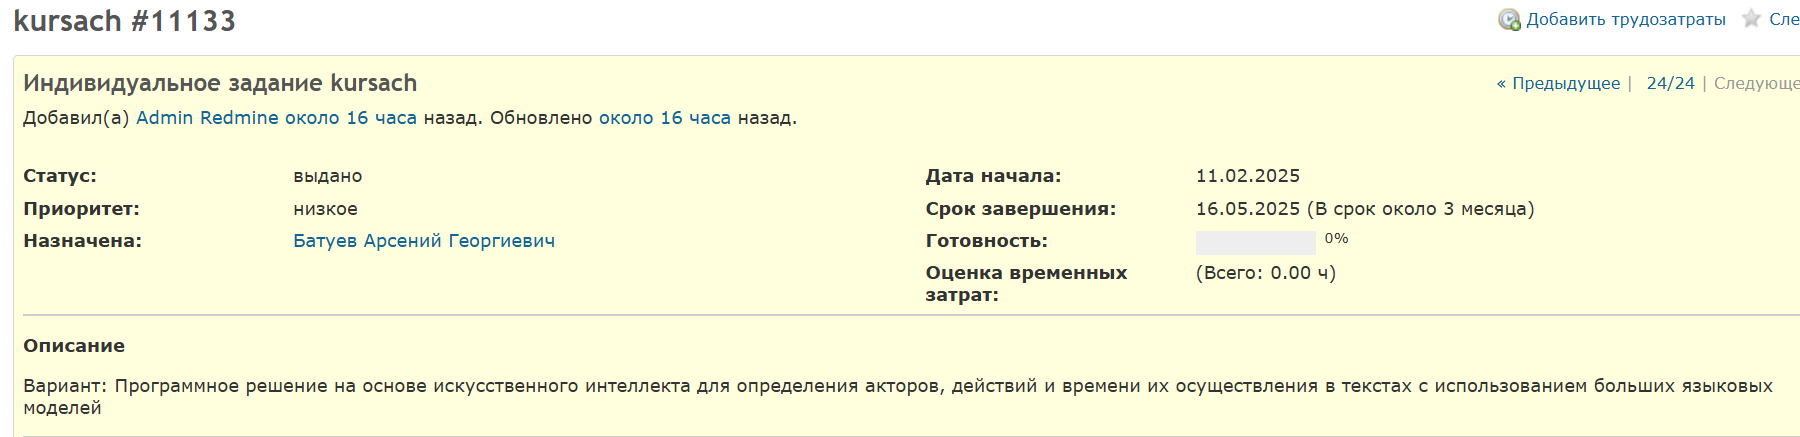
\includegraphics[width=1\linewidth]{C:/MGTU/ai_kursach/report/images/1.png}
    \caption{IDEF0 диаграмма}
\end{figure}

В рамках представленной аналитической части был проведен комплексный обзор современного состояния области извлечения информации из неструктурированных текстовых данных, с акцентом на идентификацию акторов, действий и временных характеристик

В разделе были подробно рассмотрены ключевые концепции, лежащие в основе LLM.  был проведен детальный анализ основных задач извлечения информации: распознавания именованных сущностей (NER), извлечения отношений (RE), извлечения временной информации (TIE) и извлечения событий (EE).
Обширный раздел был посвящен обзору существующих программных продуктов и платформ, реализующих функциональность извлечения информации

В совокупности, выбор модели Mistral 7b с применением 4q квантования обусловлен её способностью удовлетворять основным критериям выбора. При этом возможность применения instruct-версии модели позволяет дополнительно адаптировать её под специфические задачи, требующие точного соблюдения инструктивных параметров, что делает данное решение оптимальным для широкого спектра исследовательских и прикладных задач в области анализа текстов.

\clearpage

